\section{Experiments}
\label{sec:experiments}
In the following we briefly describe the dataset we collected for the
validation of the proposed approach. Then we describe the details of
the interactive segmentation process on those data which is depicted
in Figure\ref{fig} and we conclude with the actual timings of the
competing approaches (see Table~\ref{tab:results}).

\subsection{ALS Dataset}
\label{sec:dataset}
The data was recorded with a $3T$ scanner at
*** ANONYMISED ***.
% the Brain Institute, University of Utah.
It consisted of $12$ ALS patients and $12$ healthy controls ($64$
gradients; $b$-value$=1000$.; anatomical scan ($1 \times 1 \times
1mm^3$)).  We reconstructed the streamlines using EuDX, a
deterministic tracking algorithm ~\cite{garyfallidis2012towards} from
the DiPy library~\footnote{\url{http://www.dipy.org}}. The
tractography was then embedded in $\mathbb{R}^{p}$ using the
dissimilarity representation presented in
Section~\ref{sec:dissimilarity} with $p=40$ and the SFF prototype
selection procedure ($c=3$) as suggested
in~\cite{olivetti2012approximation}. The prototype selection and the
actual embedding of $\approx 3 \times 10^5$ streamlines required
$\approx 180$s. The resulting matrix $\phi(T) \in \mathbb{R}^{300K
  \times 40}$ was computed once and stored, so that the time to
compute the projection did not affect the interactive segmentation.


\subsection{The Interactive Segmentation Process}
We describe the segmentation process following the example of the CST
segmentation of one subject illustrated in Figure~\ref{fig}. The full
tractography (\ref{fig}A) of $\approx 250000$ streamlines was
initially clustered in $k=150$ clusters and the medoids were presented
to the user (1B). We observed that $k=150$ was approximately the
highest number of medoids the users could comfortably interact with in
the $3$D scene when the whole tractography was presented. Then user
selected $20$ clusters by clicking on the corresponding medoids
(\ref{fig}B, in white). These clusters corresponded to a set of
$\approx 15000$ streamlines (\ref{fig}C). These streamlines were
re-clustered into $k=50$ clusters (\ref{fig}D) and the user selected
$25$ of them (\ref{fig}D, in white). We observed that $50$ medoids are
approximately the highest number a user can comfortably interact with
after the initial selection from the full tractography. The $25$
selected clusters corresponds to $\approx 3000$ streamlines
(\ref{fig}E) that are then re-clustered into $k=50$ clusters
(\ref{fig}F). In two further steps the user reduced the selected
streamlines to $\approx 1500$ (\ref{fig}G) and then to $\approx 500$
(\ref{fig}I) thus reaching the desired segmentation of the CST. We
observed that a trained neuroanatomist could segment the CST in
approximately in $5$ minutes.

The average timings of the clustering algorithms of
Section~\ref{sec:methods} are reported in Table~\ref{tab:results}. In
the first column (size) are reported the size of the subset of
streamlines that were clustered. The second column ($k$) reports the
number of clusters, according to the notes expressed above. The third
($k$-means) and the fourth (MBKM) report the time for
clustering\footnote{The clustering of the whole tractography can be
  computed once and stored, so its time does not affect the
  interactive use.}. The Fifth column reports the size ($b$) of the
mini-batches for the MBKM, which was always $100$ except for the full
tractography for which we observed a significant gain in time when
increasing it to $1000$. The sixth column reports the time to compute
the medoids from the centroids provided by $k$-means and MBKM. Each
medoid was computed with simple exhaustive search within each
cluster. The time to compute all medoids was always negligible with
respect to the clustering time. All computations were performed on a
standard desktop computer.

The tractography segmentation tool was implemented in Python code on
top of the DiPy, Fos and OpenGL~\footnote{\url{http://fos.me} ,
  \url{http://opengl.org}}. The free software project of the
segmentation tool, currently in alpha stage, is hosted
*** ANONYMISED ***.
% within the DiPy project. 
The code of the dissimilarity representation is
from~\cite{olivetti2012approximation}~\footnote{\url{https://github.com/emanuele/prni2012_dissimilarity}}
and that of the $k$-means, the MBKM and the $k$-means++ is from
scikit-learn~\cite{pedregosa2011scikit}~\footnote{http://scikit-learn.org}.

\begin{figure*}[t]
\centering
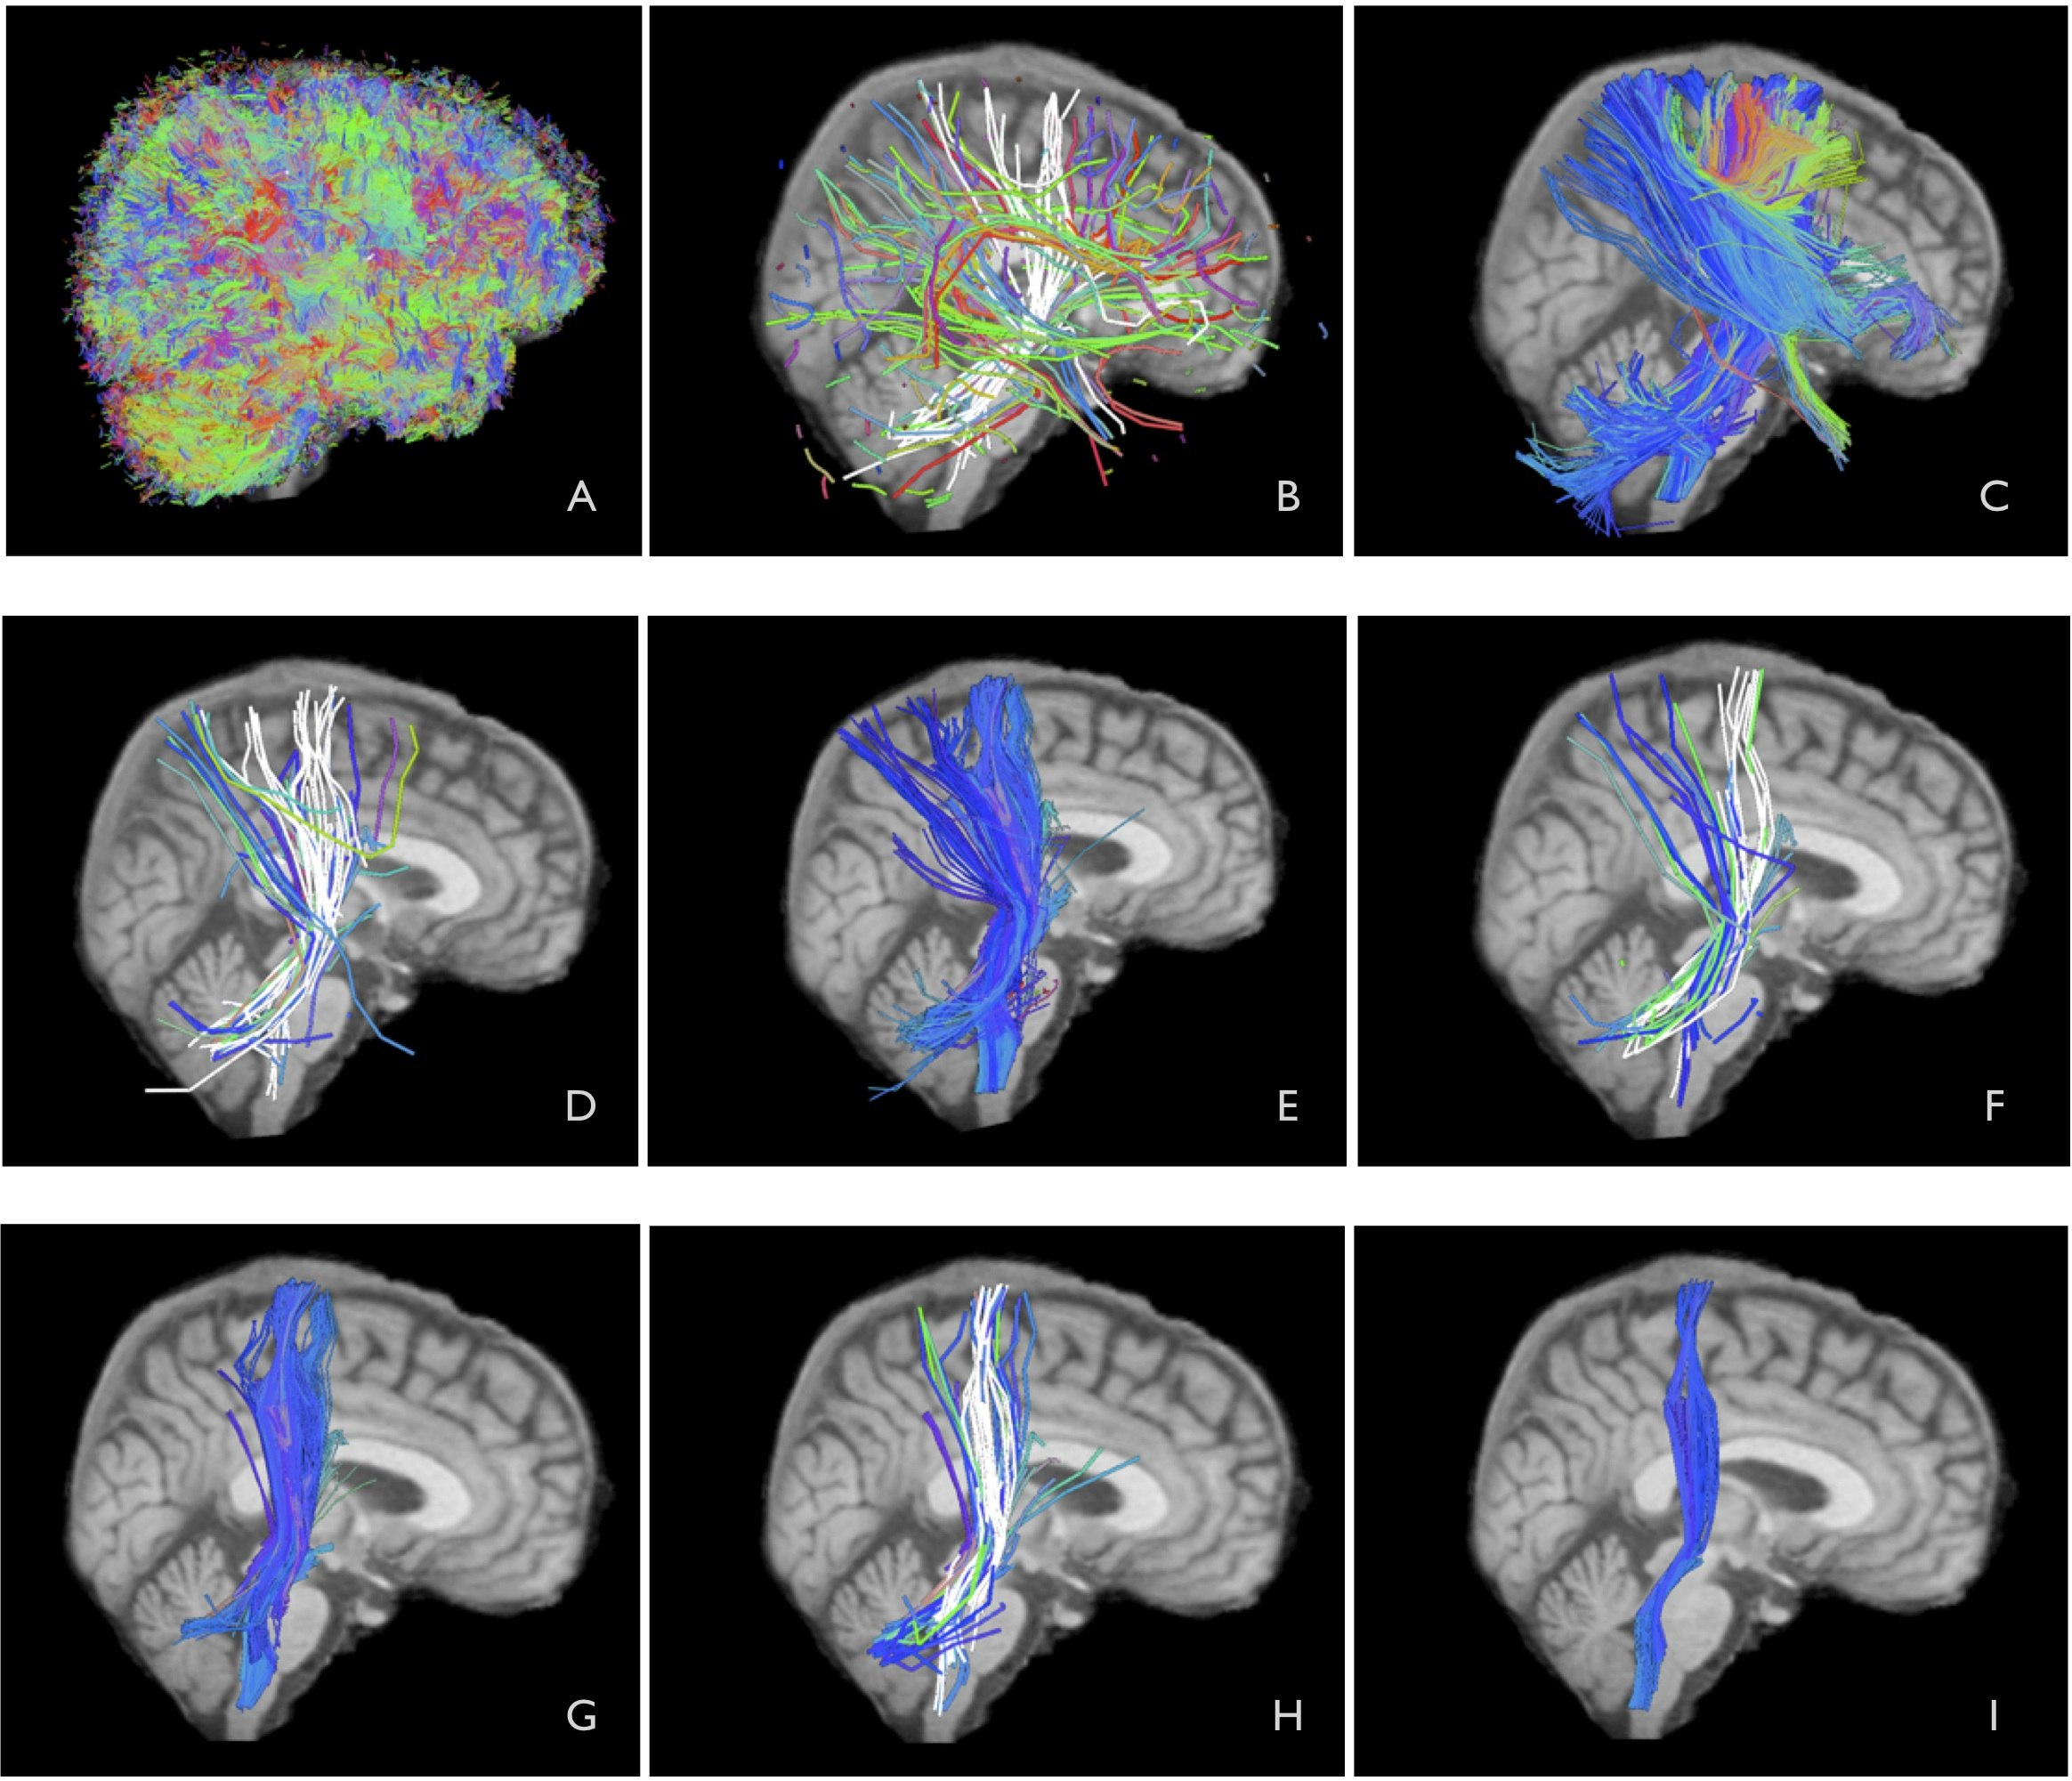
\includegraphics[width=\textwidth]{figure}
\caption{The segmentation process. (A) Full tractography $\approx 3
  \times 10^5$ streamlines; (B) Computation of 150 clusters and
  selection of 20 clusters (in white); (C) $\approx15000$ streamlines
  corresponding to previous selection; (D) Computation of 50 clusters
  and selection of 25 clusters; (E) $\approx 3000$ streamlines
  corresponding to the previous selection; (F) Computation of 50
  clusters and selection of 15 clusters; ( G) $\approx 1500$
  streamlines corresponding to the previous selection; (H) Computation
  of 50 clusters and selection of 25 clusters; (I) $\approx 500$
  streamlines corresponding to previous selection and representing the
  segmented CST.}
\label{fig}
\end{figure*}


\begin{table}
  \centering
  \begin{tabular}{ r | r || c | c || c || c }
    size & $k$ & $k$-means & MBKM & b &  medoids \\
    \hline
    \hline
    $500$    &  $50$ &  $0.3s$ &  $\mathbf{0.2}s$ &  $100$ &  $0.003s$ \\
    \hline
    $1000$   &  $50$ &  $0.6s$ &  $\mathbf{0.2}s$ &  $100$ &  $0.004s$ \\
    \hline
    $5000$   &  $50$ &  $6.1s$ &  $\mathbf{0.4}s$ &  $100$ &  $0.009s$ \\
    \hline
    $10000$  &  $50$ & $14.4s$ &  $\mathbf{0.6}s$ & $100$ &   $0.018s$ \\
    \hline
    $15000$  &  $50$ & $29.9s$ &  $\mathbf{0.7}s$ & $100$ &  $0.026s$ \\
    \hline
    $250000$ & $150$ & $>1000s$ & $\mathbf{13.3}s$ &  $1000$  &  $0.72s$ \\
    \hline
  \end{tabular}
  \caption{For a given number of streamlines (1st column, size) and a
    given number of clusters (2nd column, $k$) the time to compute the
    clustering with $k$-means and MBKM is reported in the 3rd and 4th
    columns, respectively. The size (b) of the mini-batches for MBKM is
    in the 5th column. The time to compute the medoids from the
    centroids is in the 6th column.}
  \label{tab:results}
\end{table}

%%% Local Variables: 
%%% mode: latex
%%% TeX-master: "olivetti_boi"
%%% End: 

